\documentclass[12pt, a4paper]{article}

% ── Packages ──────────────────────────────────────────────────────────────────
\usepackage[a4paper, margin=2.5cm]{geometry}
\usepackage{graphicx}
\usepackage{float}
\usepackage{amsmath}
\usepackage{amssymb}
\usepackage{xcolor}
\usepackage{mdframed}
\usepackage{parskip}
\usepackage{enumitem}
\usepackage{titlesec}
\usepackage{booktabs}
\usepackage{colortbl}
\usepackage{hyperref}
\usepackage[T1]{fontenc}
\usepackage{pgfplots}
\pgfplotsset{compat=1.18}
\usepackage{listings}
\usepackage{inconsolata}

% ── MATLAB code listing style ─────────────────────────────────────────────
\lstdefinestyle{matlab}{
  language=Matlab,
  basicstyle=\ttfamily\footnotesize,
  keywordstyle=\color{keyblue}\bfseries,
  commentstyle=\color{defgreen}\itshape,
  stringstyle=\color{noteorange},
  numberstyle=\tiny\color{black!50},
  numbers=left, numbersep=8pt,
  backgroundcolor=\color{black!4},
  frame=single, framerule=0.4pt, rulecolor=\color{black!30},
  breaklines=true, breakatwhitespace=true,
  tabsize=4, showstringspaces=false,
  morekeywords={rtccurve,rtcbdl,rtcbdu,rtcpjdu,rtcpjdl,rtcpsl,rtcpsu,
                rtcgpc,rtch,rtcv,rtcploth,rtcplotv,rtcplot,rtcplus,rtcminus,
                rtcmin,rtcmax,rtctimes,rtcfloor,rtcceil,rtcbuf,rtcdel,rtcminconv},
  xleftmargin=2em, xrightmargin=1em,
}

% ── Colours ───────────────────────────────────────────────────────────────────
\definecolor{keyblue}{RGB}{30, 80, 160}
\definecolor{keybluebg}{RGB}{220, 235, 255}
\definecolor{noteorange}{RGB}{200, 100, 0}
\definecolor{noteorangebg}{RGB}{255, 240, 215}
\definecolor{warnred}{RGB}{180, 30, 30}
\definecolor{warnredbg}{RGB}{255, 220, 220}
\definecolor{defgreen}{RGB}{20, 110, 50}
\definecolor{defgreenbg}{RGB}{215, 245, 225}
\definecolor{headernavy}{RGB}{25, 35, 90}

% ── Box environments ──────────────────────────────────────────────────────────
\newmdenv[linecolor=keyblue,backgroundcolor=keybluebg,linewidth=1.5pt,
  leftline=true,rightline=false,topline=false,bottomline=false,
  innerleftmargin=10pt,innerrightmargin=8pt,
  innertopmargin=6pt,innerbottommargin=6pt,
  skipabove=8pt,skipbelow=8pt]{keybox}

\newmdenv[linecolor=noteorange,backgroundcolor=noteorangebg,linewidth=1.5pt,
  leftline=true,rightline=false,topline=false,bottomline=false,
  innerleftmargin=10pt,innerrightmargin=8pt,
  innertopmargin=6pt,innerbottommargin=6pt,
  skipabove=8pt,skipbelow=8pt]{notebox}

\newmdenv[linecolor=warnred,backgroundcolor=warnredbg,linewidth=1.5pt,
  leftline=true,rightline=false,topline=false,bottomline=false,
  innerleftmargin=10pt,innerrightmargin=8pt,
  innertopmargin=6pt,innerbottommargin=6pt,
  skipabove=8pt,skipbelow=8pt]{warnbox}

\newmdenv[linecolor=defgreen,backgroundcolor=defgreenbg,linewidth=1.5pt,
  leftline=true,rightline=false,topline=false,bottomline=false,
  innerleftmargin=10pt,innerrightmargin=8pt,
  innertopmargin=6pt,innerbottommargin=6pt,
  skipabove=8pt,skipbelow=8pt]{defbox}

% ── Section formatting ────────────────────────────────────────────────────────
\titleformat{\section}[block]{\large\bfseries\color{headernavy}}{}{0pt}{}
  [\vspace{2pt}\rule{\linewidth}{0.8pt}\vspace{4pt}]
\titleformat{\subsection}[block]{\normalsize\bfseries\color{keyblue}}{}{0pt}{}

% ── Document ──────────────────────────────────────────────────────────────────
\begin{document}

\begin{center}
  {\LARGE\bfseries\color{headernavy} Networks and Systems}\\[4pt]
  {\large Lectures 4 \& 5 --- Exercise 1: Sensor Network Packetisation}\\[2pt]
  {\normalsize Network Performance Analysis \quad|\quad Electronic Systems, 8th Semester}
\end{center}

\vspace{4pt}\hrule height 1.2pt\vspace{12pt}

% ==============================================================================
\section*{Problem Statement}
% ==============================================================================

\begin{notebox}
\textbf{Note on notation.}
The original exercise statement uses the letter $N$ for two distinct things: the
number of sensors (which is a fixed given value of 8) and the number of data
points per packet (which is the quantity to be determined). To avoid confusion,
this document uses $n_s = 8$ for the number of sensors, and reserves $N$ solely
for the number of data points bundled into each packet.
\end{notebox}

\vspace{4pt}
A sensor network consists of $n_s = 8$ identical sensors sharing a single
communication link. The setup is as follows:

\begin{itemize}[leftmargin=1.4em, itemsep=4pt]
  \item Each sensor generates \textbf{100 bits} of measurement data periodically,
    once every $T = 1\,\mathrm{ms}$.
  \item All sensors share a single communication line with a serialisation speed
    (link bandwidth) of $s = 1\,\mathrm{Mbps} = 1000\,\mathrm{kbps}$.
  \item Before transmission, each sensor \textbf{buffers} $N$ consecutive data
    samples and then sends them as a single packet. Each packet consists of the
    $N$ data samples (each 100 bits) plus a fixed overhead (header, error
    detection, etc.) of $O = 100\,\mathrm{bits}$.
\end{itemize}

\textbf{Tasks:}
\begin{enumerate}[leftmargin=1.6em, itemsep=4pt]
  \item Determine the \textbf{optimal value of $N$} --- the number of data points
    per packet --- taking into account both the end-to-end delay experienced by
    the data and the bandwidth utilisation of the shared link.
  \item For an \textbf{arbitrary $N$}, derive the \textbf{DNC arrival constraint}
    (arrival curve) for a single sensor, and then the \textbf{aggregate arrival
    curve} for all $n_s = 8$ sensors combined.
\end{enumerate}

% ==============================================================================
\section*{Background: Why Does $N$ Matter?}
% ==============================================================================

The choice of $N$ controls a fundamental trade-off in packetised sensor
networks.

\textbf{Large $N$:}
\begin{itemize}[leftmargin=1.4em, itemsep=2pt]
  \item Each packet carries more data, so the overhead $O = 100\,\mathrm{bits}$
    is spread over more payload bytes.
    The \emph{overhead fraction} $O/L = 100/[100(N+1)] = 1/(N+1)$ shrinks,
    meaning the link is used more efficiently (less bandwidth wasted on headers).
  \item However, a sensor must wait longer before it has accumulated $N$ samples.
    The most recently generated data point sits in the buffer for up to
    $(N-1) \times T$ milliseconds before the packet is sent.
    \textbf{Delay increases.}
\end{itemize}

\textbf{Small $N$:}
\begin{itemize}[leftmargin=1.4em, itemsep=2pt]
  \item Packets are sent more frequently and contain fewer samples, so individual
    data points are transmitted sooner. \textbf{Delay decreases.}
  \item But each packet carries a large overhead relative to its payload. More
    packets per second means more overhead bytes per second, consuming a larger
    share of the link capacity. If $N$ is too small the total offered load exceeds
    the link bandwidth and the system becomes \textbf{unstable} (infinite queues).
\end{itemize}

Both the bandwidth and delay depend on $N$ in opposite directions --- the
solution is to find the smallest $N$ that keeps the system stable, since that
also minimises delay.

% ==============================================================================
\section*{Task 1 --- Optimal Packet Size $N$}
% ==============================================================================

% ------------------------------------------------------------------------------
\subsection*{Step 1: Derive the packet length $L$}
% ------------------------------------------------------------------------------

Each packet from one sensor contains $N$ data samples of 100 bits each, plus
$O = 100\,\mathrm{bits}$ of overhead:
\[
  L = N \times 100 + O = 100N + 100 = 100(N+1) \quad \text{[bits]}.
\]
\begin{itemize}[leftmargin=1.4em, itemsep=2pt]
  \item $L$ --- total packet length in bits.
  \item $N$ --- number of data samples bundled per packet (to be determined).
  \item $100$ bits --- size of one data sample.
  \item $O = 100$ bits --- fixed overhead (header, error detection, etc.).
\end{itemize}

% ------------------------------------------------------------------------------
\subsection*{Step 2: Find the inter-packet period $P$}
% ------------------------------------------------------------------------------

Because a sensor generates one sample every $T = 1\,\mathrm{ms}$ and must
collect $N$ samples before sending, the inter-packet period is:
\[
  P = N \times T = N \times 1\,\mathrm{ms} = N\,\mathrm{ms}.
\]
\begin{itemize}[leftmargin=1.4em, itemsep=2pt]
  \item $P$ --- time between successive packet transmissions from one sensor.
  \item $N$ --- the buffering window (number of samples to collect).
  \item $T = 1\,\mathrm{ms}$ --- sampling period of each sensor.
\end{itemize}

% ------------------------------------------------------------------------------
\subsection*{Step 3: Bandwidth constraint}
% ------------------------------------------------------------------------------

Each of the $n_s = 8$ sensors sends one packet of $L$ bits every $P$ ms. The
total offered bit rate to the shared link is:
\[
  r_\text{total} = n_s \cdot \frac{L}{P}
  = 8 \cdot \frac{100(N+1)}{N\,\mathrm{ms}}
  = \frac{800(N+1)}{N}\,\mathrm{kbps}.
\]
\begin{itemize}[leftmargin=1.4em, itemsep=2pt]
  \item $r_\text{total}$ --- total bit rate offered to the link by all sensors.
  \item $n_s = 8$ --- number of sensors.
  \item $L = 100(N+1)$ bits --- packet size.
  \item $P = N\,\mathrm{ms}$ --- inter-packet period per sensor.
\end{itemize}

For the link not to become overloaded, the offered rate must not exceed the
link speed. The utilisation $\rho$ must satisfy:
\[
  \rho = \frac{r_\text{total}}{s} = \frac{800(N+1)}{N \times 1000} = \frac{0.8(N+1)}{N} \leq 1.
\]
\begin{itemize}[leftmargin=1.4em, itemsep=2pt]
  \item $\rho$ --- link utilisation (dimensionless); must be at most 1 for the
    offered load not to exceed link capacity.
  \item $s = 1000\,\mathrm{kbps}$ --- link capacity.
\end{itemize}

Solving for $N$:
\[
  \frac{0.8(N+1)}{N} \leq 1
  \;\Longrightarrow\;
  0.8N + 0.8 \leq N
  \;\Longrightarrow\;
  0.8 \leq 0.2N
  \;\Longrightarrow\;
  N \geq 4.
\]

So the minimum integer satisfying the bandwidth constraint is $N = 4$, which
gives exactly $\rho = 0.8 \times 5/4 = 1.0$ --- the link is fully utilised.
Under the idealised assumption of this exercise (perfectly periodic sensors,
no jitter, no burst) this is mathematically valid: the offered rate equals the
capacity and the link can just keep up.

\begin{warnbox}
  \textbf{$N = 4$ works in theory, but is not recommended in practice.}

  Designing to $\rho = 1.0$ means the link has \textbf{zero spare capacity}.
  In any realistic system this is problematic:
  \begin{itemize}[leftmargin=1.2em, itemsep=2pt]
    \item Sensors are not perfectly synchronised --- small timing jitter means
      packets from multiple sensors can collide at the link simultaneously,
      creating momentary bursts that exceed the link rate and causing queues
      to grow.
    \item Any other background traffic (management frames, retransmissions)
      instantly pushes utilisation above 1 and the queue grows without bound.
    \item Clock drift over time means the ``perfectly periodic'' assumption
      gradually breaks down.
  \end{itemize}
  For these reasons, a utilisation of $\rho = 1.0$ is not a robust operating
  point. The next valid value, $N = 5$ ($\rho = 0.96$), provides a small but
  meaningful safety margin and is the \textbf{recommended practical choice}.
\end{warnbox}

\clearpage
% ------------------------------------------------------------------------------
\subsection*{Step 4: Worst-case end-to-end delay}
% ------------------------------------------------------------------------------

The total delay a data sample experiences has three additive components:

\textbf{(a) Packetisation delay $d_\text{pkt}$:}
A data sample generated at the very start of a collection window must wait
for the remaining $N-1$ samples to arrive before the packet can be dispatched:
\[
  d_\text{pkt} = (N-1) \times T = (N-1)\,\mathrm{ms}.
\]

\textbf{(b) Queuing delay $d_\text{queue}$:}
In the worst case, all other $n_s - 1 = 7$ sensors happen to finish their
collection windows at the same time and also have a packet ready. Our packet
must wait for each of those 7 packets to be transmitted before it can start:
\[
  d_\text{queue} = 7 \times \frac{L}{s}
  = 7 \times \frac{100(N+1)}{1000}\,\mathrm{ms}
  = 0.7(N+1)\,\mathrm{ms}.
\]

\textbf{(c) Serialisation delay $d_\text{ser}$:}
The time to push the packet itself onto the wire:
\[
  d_\text{ser} = \frac{L}{s}
  = \frac{100(N+1)}{1000}\,\mathrm{ms}
  = 0.1(N+1)\,\mathrm{ms}.
\]

Total worst-case end-to-end delay:
\[
  D(N) = d_\text{pkt} + d_\text{queue} + d_\text{ser}
  = (N-1) + 0.7(N+1) + 0.1(N+1)
  = (N-1) + 0.8(N+1).
\]

Expanding:
\[
  \boxed{D(N) = 1.8N - 0.2 \quad [\mathrm{ms}].}
\]
\begin{itemize}[leftmargin=1.4em, itemsep=2pt]
  \item $D(N)$ --- worst-case delay in milliseconds as a function of $N$.
  \item The coefficient $1.8$ and constant $-0.2$ come from combining the three
    delay terms above.
  \item $D(N)$ is \textbf{strictly increasing} in $N$: every extra data point
    bundled into a packet adds 1.8\,ms to the worst-case delay.
\end{itemize}

% ------------------------------------------------------------------------------
\subsection*{Step 5: Determine the optimal $N$}
% ------------------------------------------------------------------------------

We now have two constraints pulling in opposite directions:

\begin{center}
\begin{tabular}{lccc}
\toprule
$N$ & $\rho = 0.8(N+1)/N$ & Stable? & $D(N)$ [ms] \\
\midrule
1 & 1.60 & \textbf{No}  & 1.6  \\
2 & 1.20 & \textbf{No}  & 3.4  \\
3 & 1.07 & \textbf{No}  & 5.2  \\
\rowcolor{keybluebg}
4 & 1.00 & Yes --- $\rho=1$ (theoretical min.) & 7.0  \\
\rowcolor{defgreenbg}
5 & 0.96 & \textbf{Yes --- recommended} & 8.8  \\
6 & 0.93 & Yes & 10.6 \\
7 & 0.91 & Yes & 12.4 \\
8 & 0.90 & Yes & 14.2 \\
\bottomrule
\end{tabular}
\end{center}

\begin{keybox}
  \textbf{Theoretical minimum: $N = 4$ \quad ($\rho = 1.0$, lowest delay
  satisfying the bandwidth constraint).}
  \begin{itemize}[leftmargin=1.2em, itemsep=2pt]
    \item Packet size: $L = 100 \times 5 = 500\,\mathrm{bits}$
    \item Inter-packet period per sensor: $P = 4\,\mathrm{ms}$
    \item Link utilisation: $\rho = 1.00$ (link fully loaded)
    \item Worst-case delay: $D(4) = 7.0\,\mathrm{ms}$
  \end{itemize}

  \textbf{Practical recommendation: $N = 5$} --- avoids the zero-headroom
  problem at $\rho = 1$ while adding only $1.8\,\mathrm{ms}$ of extra delay.
  \begin{itemize}[leftmargin=1.2em, itemsep=2pt]
    \item Packet size: $L = 100 \times 6 = 600\,\mathrm{bits}$
    \item Inter-packet period per sensor: $P = 5\,\mathrm{ms}$
    \item Link utilisation: $\rho = 0.96$
    \item Worst-case delay: $D(5) = 8.8\,\mathrm{ms}$
  \end{itemize}
\end{keybox}

The figure below shows utilisation and delay versus $N$. Both $N=4$ (blue
highlight, $\rho = 1.0$) and $N = 5$ (green highlight, recommended) are marked.

\begin{figure}[H]
\centering
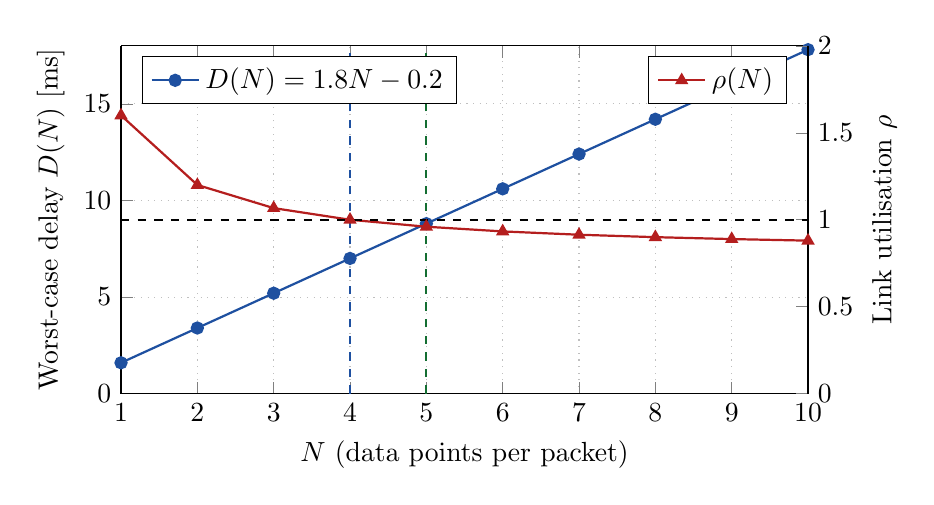
\begin{tikzpicture}
\begin{axis}[
  width=0.85\textwidth, height=6cm,
  xlabel={$N$ (data points per packet)},
  ylabel={Worst-case delay $D(N)$ [ms]},
  axis y line*=left,
  xmin=1, xmax=10, ymin=0, ymax=18,
  xtick={1,2,...,10},
  grid=major, grid style={dotted, gray!50},
  legend pos=north west,
]
\addplot[thick, color=keyblue, mark=*, mark size=2pt]
  coordinates {(1,1.6)(2,3.4)(3,5.2)(4,7.0)(5,8.8)(6,10.6)(7,12.4)(8,14.2)(9,16.0)(10,17.8)};
\addlegendentry{$D(N)=1.8N-0.2$}
\addplot[dashed, thick, color=keyblue, forget plot]
  coordinates {(4,0)(4,18)};
\addplot[dashed, thick, color=defgreen, forget plot]
  coordinates {(5,0)(5,18)};
\end{axis}
\begin{axis}[
  width=0.85\textwidth, height=6cm,
  ylabel={Link utilisation $\rho$},
  axis y line*=right,
  axis x line=none,
  xmin=1, xmax=10, ymin=0, ymax=2.0,
  ytick={0, 0.5, 1.0, 1.5, 2.0},
  legend pos=north east,
]
\addplot[thick, color=warnred, mark=triangle*, mark size=2pt]
  coordinates {(1,1.6)(2,1.2)(3,1.067)(4,1.0)(5,0.96)(6,0.933)(7,0.914)(8,0.9)(9,0.889)(10,0.88)};
\addlegendentry{$\rho(N)$}
\addplot[dashed, color=black, thick, forget plot]
  coordinates {(1,1.0)(10,1.0)};
\end{axis}
\end{tikzpicture}
\caption{Delay $D(N)$ (blue curve, left axis) and utilisation $\rho(N)$ (red
  curve, right axis) as a function of $N$. The black dashed horizontal line
  marks $\rho = 1$.
  The \textbf{blue vertical dashed} line marks $N = 4$: the theoretical
  minimum satisfying $\rho \leq 1$ (link exactly fully loaded).
  The \textbf{green vertical dashed} line marks $N = 5$: the recommended
  practical choice with a small headroom ($\rho = 0.96$).
  For $N \leq 3$ the offered load exceeds the link capacity.}
\end{figure}

% ==============================================================================
\section*{Task 2 --- DNC Arrival Curves}
% ==============================================================================

Deterministic Network Calculus (DNC) characterises traffic flows using
\textbf{arrival curves}. An arrival curve $\alpha(t)$ is an upper bound on the
amount of data any flow can inject into the network in any time window of
length $t$:
\[
  A(s, s+t) \leq \alpha(t) \quad \forall\, s \geq 0,\; t \geq 0,
\]
\begin{itemize}[leftmargin=1.4em, itemsep=2pt]
  \item $A(s, s+t)$ --- number of bits arriving in the interval $(s,\, s+t]$.
  \item $\alpha(t)$ --- the arrival curve: a non-decreasing function bounding
    the worst-case arrivals in any window of length $t$.
\end{itemize}

The most common arrival curve model is the \textbf{token bucket} (also called
leaky bucket), written $\alpha(t) = r \cdot t + b$, where:
\begin{itemize}[leftmargin=1.4em, itemsep=2pt]
  \item $r$ --- the \textbf{token rate} (long-term average rate); tokens
    accumulate in a bucket at rate $r$ and each bit of data consumes one token.
    This bounds how fast data can be sent in a sustained way.
  \item $b$ --- the \textbf{bucket size} (burst parameter); the maximum number
    of bits that can be sent instantaneously (i.e.\ the maximum burst in any
    arbitrarily short window).
\end{itemize}

% ------------------------------------------------------------------------------
\subsection*{Single-sensor arrival curve}
% ------------------------------------------------------------------------------

Each sensor is a \textbf{periodic on-off source}: it is silent for $P = N$\,ms
while buffering samples, then injects one packet of $L = 100(N+1)$ bits all
at once, then is silent again for another $P$ ms.

The tightest token-bucket arrival curve for this source is found by asking:
\emph{what is the maximum number of bits this sensor can send in any window of
length $t$?}

\begin{itemize}[leftmargin=1.4em, itemsep=4pt]
  \item \textbf{Burst $b$:} In any arbitrarily short window ($t \to 0$), the
    worst case is one packet arriving all at once:
    \[
      b = L = 100(N+1)\,\mathrm{bits}.
    \]
  \item \textbf{Rate $r$:} Over a long window the average sending rate is one
    packet per period:
    \[
      r = \frac{L}{P} = \frac{100(N+1)}{N\,\mathrm{ms}}
        = \frac{100(N+1)}{N}\,\mathrm{kbps}.
    \]
\end{itemize}

The single-sensor arrival curve is therefore:
\[
  \boxed{\alpha_s(t) = \frac{100(N+1)}{N}\cdot t + 100(N+1) \quad
  \text{[bits, with $t$ in ms]}.}
\]
\begin{itemize}[leftmargin=1.4em, itemsep=2pt]
  \item $\alpha_s(t)$ --- worst-case bits sent by one sensor in any interval of
    length $t$.
  \item $\frac{100(N+1)}{N}$ --- token rate in kbps (bits per ms); the
    sustainable long-term rate of the sensor.
  \item $100(N+1)$ bits --- burst size; one full packet can arrive
    instantaneously.
\end{itemize}

\begin{notebox}
  \textbf{Physical meaning of $b$ and $r \cdot t$ in the token bucket.}

  \textbf{The burst term $b$} represents the worst-case instantaneous injection
  of bits --- the amount of data that can arrive in an arbitrarily short window.
  For our sensor this is exactly one full packet $L$, because the sensor
  accumulates $N$ samples silently and then sends them all at once.
  Concretely: imagine the link briefly goes down and then recovers.
  While the link was down, the sensor kept generating samples and filling its
  buffer. The moment the link comes back, a fully-loaded packet ($L$ bits) is
  released instantly. The bucket size $b = L$ bounds exactly this burst.

  \textbf{The rate term $r \cdot t$} represents the ongoing, sustained
  accumulation of data over time. After the initial burst, the sensor keeps
  generating one data point every $T = 1\,\mathrm{ms}$, so data accumulates
  at the long-term rate $r = L/P$. Over a window of length $t$ at most
  $r \cdot t$ additional bits can be produced, regardless of when in that
  window they arrive.

  Together, $\alpha_s(t) = r \cdot t + b$ says: \emph{in any time window of
  length $t$, a single sensor sends at most $b$ bits as an initial burst plus
  $r \cdot t$ bits from sustained generation.}
\end{notebox}

% ------------------------------------------------------------------------------
\subsection*{Aggregate arrival curve for all $n_s = 8$ sensors}
% ------------------------------------------------------------------------------

When multiple flows share a link, DNC computes the aggregate arrival curve by
\textbf{summing} the individual arrival curves. This is a valid (worst-case)
bound because at any given moment each sensor could independently be at the
peak of its burst:
\[
  \alpha_\text{agg}(t) = \sum_{k=1}^{n_s} \alpha_s(t) = n_s \cdot \alpha_s(t).
\]

Since all 8 sensors are identical:
\[
  \alpha_\text{agg}(t) = 8 \cdot \left[\frac{100(N+1)}{N}\cdot t + 100(N+1)\right].
\]

\[
  \boxed{\alpha_\text{agg}(t) = \frac{800(N+1)}{N}\cdot t + 800(N+1)
  \quad \text{[bits, with $t$ in ms]}.}
\]
\begin{itemize}[leftmargin=1.4em, itemsep=2pt]
  \item $\frac{800(N+1)}{N}$ --- aggregate token rate in kbps; the total
    long-term rate offered to the link by all 8 sensors. This is exactly
    $r_\text{total}$ from Task~1.
  \item $800(N+1)$ bits --- aggregate burst; the maximum number of bits that
    could arrive simultaneously if all 8 sensors released a packet at the
    exact same instant.
\end{itemize}

\begin{notebox}
  \textbf{Consistency check --- using $N = 4$ (the theoretical answer).}
  Substituting $N = 4$: aggregate rate $= 800 \times 5/4 = 1000\,\mathrm{kbps} = s$,
  aggregate burst $= 800 \times 5 = 4000\,\mathrm{bits}$.
  The aggregate arrival rate \emph{exactly equals} the link speed, which is
  consistent with $\rho = 1.0$ from Task~1.
\end{notebox}

\vspace{4pt}
For $N = 4$, the aggregate arrival curve and the link's \textbf{service curve}
$\beta(t) = s \cdot t = 1000\,t$ can be compared directly.

At $t = 0$ the arrival curve starts $b_\text{agg} = 4000\,\mathrm{bits}$ above
the service curve --- the worst-case burst from all 8 sensors releasing
simultaneously.
This is the maximum backlog the link must absorb.

After $t = 0$, however, the two curves rise at \emph{exactly the same slope}:
\[
  r_\text{agg} = \frac{800(N+1)}{N}\Big|_{N=4} = \frac{800 \times 5}{4}
  = 1000\,\mathrm{kbps} = s.
\]
The net drain rate is therefore:
\[
  s - r_\text{agg} = 1000 - 1000 = 0\,\mathrm{kbps}.
\]
The two curves are \textbf{parallel} --- the gap never closes.
Setting $\beta(t^*) = \alpha_\text{agg}(t^*)$:
\[
  1000\,t^* = 1000\,t^* + 4000
  \;\Longrightarrow\;
  0 = 4000
  \;\Longrightarrow\;
  \boxed{t^* = \infty.}
\]
The service curve \emph{never catches up} to the arrival curve.
Any burst that enters the queue at $N = 4$ stays there permanently.
This is the graphical confirmation of what the warnbox in Task~1 stated: a
utilisation of exactly 1 means the system has zero capacity to absorb bursts.

\begin{figure}[H]
\centering
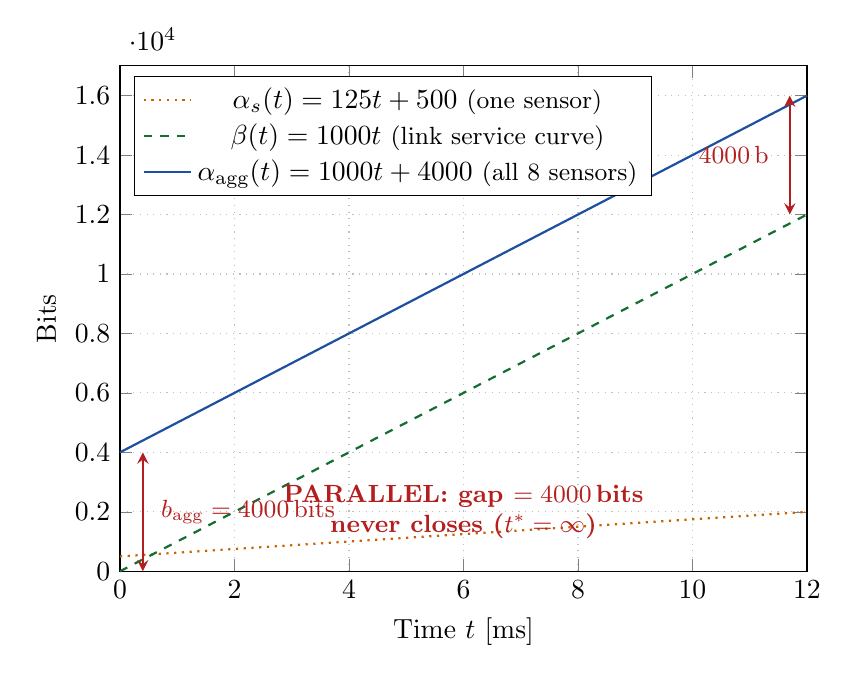
\begin{tikzpicture}
\begin{axis}[
  width=0.85\textwidth, height=8cm,
  xlabel={Time $t$ [ms]},
  ylabel={Bits},
  xmin=0, xmax=12, ymin=0, ymax=17000,
  grid=major, grid style={dotted, gray!50},
  legend style={at={(0.02,0.98)}, anchor=north west},
  clip=false,
]
% Single sensor curve: alpha_s(t) = 125*t + 500  (N=4)
\addplot[thick, dotted, color=noteorange, domain=0:12, samples=2]
  {125*x + 500};
\addlegendentry{$\alpha_s(t) = 125t + 500$ \small(one sensor)}

% Service curve: beta(t) = 1000*t
\addplot[thick, dashed, color=defgreen, domain=0:12, samples=2]
  {1000*x};
\addlegendentry{$\beta(t) = 1000t$ \small(link service curve)}

% Aggregate arrival curve: alpha_agg(t) = 1000*t + 4000  (N=4)
\addplot[thick, color=keyblue, domain=0:12, samples=2]
  {1000*x + 4000};
\addlegendentry{$\alpha_\text{agg}(t) = 1000t + 4000$ \small(all 8 sensors)}

% --- Annotate the burst b_agg = 4000 bits at t=0 ---
\addplot[<->, >=stealth, thick, color=warnred]
  coordinates {(0.4, 0)(0.4, 4000)};
\node[right, color=warnred, font=\small] at (axis cs:0.55, 2000)
  {$b_\text{agg}=4000\,\text{bits}$};

% --- Annotate constant gap at t=12 ---
% alpha_agg(12) = 12000+4000 = 16000, beta(12) = 12000, gap = 4000
\addplot[<->, >=stealth, thick, color=warnred]
  coordinates {(11.7, 12000)(11.7, 16000)};
\node[left, color=warnred, font=\small] at (axis cs:11.5, 14000)
  {$4000\,\text{b}$};

% --- PARALLEL label ---
\node[color=warnred, font=\small\bfseries, align=center]
  at (axis cs:6, 2000)
  {PARALLEL: gap $= 4000\,\text{bits}$\\never closes ($t^* = \infty$)};

\end{axis}
\end{tikzpicture}
\caption{DNC arrival and service curves for $N=4$ ($\rho = 1.0$).
  The \textbf{blue solid} line ($\alpha_\text{agg} = 1000t + 4000$) and the
  \textbf{green dashed} line ($\beta = 1000t$) have \emph{identical slopes} ---
  they are parallel.
  The vertical gap of $b_\text{agg} = 4000\,\mathrm{bits}$ (red arrows) is
  constant for all $t$: the link can never drain the burst backlog.
  Any worst-case burst that occurs at $N=4$ is permanent.
  The \textbf{orange dotted} line is a single sensor's arrival curve.}
\end{figure}

% ------------------------------------------------------------------------------
\subsection*{What the arrival/service curve figure tells us}
% ------------------------------------------------------------------------------

\begin{keybox}
  \textbf{Reading the DNC curve --- key numbers for $N = 4$:}

  \begin{enumerate}[leftmargin=1.6em, itemsep=6pt]

    \item \textbf{Maximum backlog} $= b_\text{agg} = 800(N+1)\big|_{N=4} = 4000\,\text{bits}$

      This is the vertical gap at $t = 0$: the worst-case burst when all 8
      sensors fire simultaneously (e.g.\ right after a brief link hiccup lasting
      less than $P = 4\,\text{ms}$).
      The link needs $4000/1000 = 4\,\text{ms}$ of transmission time just to
      clear this burst --- and at $N=4$ it \emph{never gets the chance to}.

    \item \textbf{Net drain rate} $= s - r_\text{agg} = 1000 - 1000 = 0\,\text{kbps}$

      Both curves have slope $1000\,\text{kbps}$.
      There is zero spare capacity; the link is fully occupied just keeping up
      with the steady-state traffic and has nothing left to drain a burst.

    \item \textbf{Time to clear the burst} $= t^* = b_\text{agg} / (s - r_\text{agg}) = 4000/0 = \infty$

      The gap never closes. If a burst of $4000\,\text{bits}$ ever forms in the
      queue, it stays there forever. The figure makes this visible: the red gap
      arrows are the \emph{same size} at $t=0$ and $t=12\,\text{ms}$.

    \item \textbf{Maximum delay per packet} $= b_\text{agg}/s = 4000/1000 = 4\,\text{ms}$

      In DNC the worst-case queuing delay equals $b/s$ (the horizontal distance
      between the two curves).
      A packet arriving behind a full $4000$-bit burst queue must wait
      $4\,\text{ms}$ for it to drain, plus $L/s = 500/1000 = 0.5\,\text{ms}$
      for its own serialisation. Adding the packetisation delay
      $d_\text{pkt} = 3\,\text{ms}$ gives a total worst-case delay of
      $7.5\,\text{ms}$ --- which is consistent with (and slightly above) the
      $D(4) = 7.0\,\text{ms}$ from Task~1.

  \end{enumerate}

  \vspace{6pt}
  \textbf{Why this argues for $N = 5$.}
  Switching from $N = 4$ to $N = 5$ changes $r_\text{agg}$ from
  $1000\,\text{kbps}$ to $960\,\text{kbps}$, giving a net drain rate of
  $40\,\text{kbps}$ instead of zero.
  The burst is now cleared in $t^* = 4800/40 = 120\,\text{ms}$ instead of
  never. The cost is $1.8\,\text{ms}$ of extra end-to-end delay.
  That trade-off --- $120\,\text{ms}$ burst recovery time versus
  $1.8\,\text{ms}$ extra latency --- is what makes $N = 5$ the
  practical recommendation.
\end{keybox}

% ==============================================================================
\section*{Summary}
% ==============================================================================

\begin{keybox}
\textbf{Task 1 --- Optimal packet size:}

\vspace{4pt}
Packet length: $L = 100(N+1)$ bits. \quad
Inter-packet period per sensor: $P = N\,\mathrm{ms}$.

\vspace{4pt}
Bandwidth constraint: $\rho = \dfrac{0.8(N+1)}{N} \leq 1 \;\Rightarrow\; N \geq 4$.

\vspace{4pt}
Worst-case delay: $D(N) = 1.8N - 0.2\,\mathrm{ms}$ --- strictly increasing in $N$.

\vspace{4pt}
$\Rightarrow$ \textbf{Theoretical answer: $N = 4$} \; ($\rho = 1.0$, $D = 7.0\,\mathrm{ms}$).
Under the idealised assumptions of the exercise (perfectly periodic, no jitter)
this satisfies the constraint with minimum delay.

\vspace{4pt}
$\Rightarrow$ \textbf{Practical recommendation: $N = 5$} \; ($\rho = 0.96$, $D =
8.8\,\mathrm{ms}$). Designing to $\rho = 1$ leaves no headroom for jitter,
timing imperfections, or any other traffic; $N = 5$ adds only $1.8\,\mathrm{ms}$
of delay while providing a meaningful safety margin.
\end{keybox}

\begin{keybox}
\textbf{Task 2 --- DNC arrival curves (general $N$):}

\vspace{4pt}
Single sensor (token bucket $\alpha = r \cdot t + b$):
\[
  \alpha_s(t) = \frac{100(N+1)}{N}\,t + 100(N+1)
  \quad \text{[bits, $t$ in ms]}
\]

\vspace{4pt}
Aggregate for all 8 sensors:
\[
  \alpha_\text{agg}(t) = \frac{800(N+1)}{N}\,t + 800(N+1)
  \quad \text{[bits, $t$ in ms]}
\]

\vspace{4pt}
For $N = 4$ (theoretical answer):
$\alpha_s(t) = 125\,t + 500$ and
$\alpha_\text{agg}(t) = 1000\,t + 4000$. \\
Curves \textbf{parallel} to service curve $\beta = 1000t$ --- burst never drains ($t^* = \infty$).

\vspace{4pt}
For $N = 5$ (practical recommendation):
$\alpha_s(t) = 120\,t + 600$ and
$\alpha_\text{agg}(t) = 960\,t + 4800$. \\
Net drain rate $= 40\,\text{kbps}$, burst clears after $t^* = 120\,\text{ms}$.
\end{keybox}

% ==============================================================================
\newpage
\section*{Exercise 2 \quad RTC Toolbox Analysis of the Sensor Network}
% ==============================================================================

\begin{notebox}
  \textbf{Note --- this exercise is entirely code-based.}
  All results are computed by the RTC Toolbox running in MATLAB.
  The code file is \texttt{ex2\_rtc.m} in the same folder.
  Before running it, ensure the toolbox is installed and call \texttt{rtc\_init}
  to load the Java kernel.
\end{notebox}

% ------------------------------------------------------------------------------
\subsection*{Problem Statement}
% ------------------------------------------------------------------------------

Using the RTC Toolbox, encode the arrival and service curves derived in Exercise~1
and use them to compute delay and backlog bounds programmatically.
Specifically:

\begin{enumerate}[leftmargin=1.6em, itemsep=4pt]
  \item Encode the aggregated arrival constraint for all 8~sensors as an
    \texttt{rtccurve} object.
  \item Encode the service curve of the communication link using the
    toolbox (the lower bounded-delay service curve).
  \item Use \texttt{rtch} and \texttt{rtcploth} to compute and plot the
    worst-case \textbf{delay} bound.
  \item Use \texttt{rtcv} and \texttt{rtcplotv} to compute and plot the
    worst-case \textbf{backlog} bound.
  \item Use an appropriate sweep over $N$ with \texttt{rtch} to identify the
    optimal value of $N$.
\end{enumerate}

% ------------------------------------------------------------------------------
\subsection*{RTC Toolbox Functions Used}
% ------------------------------------------------------------------------------

\begin{defbox}
  \textbf{Key functions in this exercise:}
  \begin{itemize}[leftmargin=1.2em, itemsep=4pt]
    \item \texttt{rtccurve([[x0\ y0\ slope; ...]])} --- creates an
      arbitrary piecewise-linear curve from a matrix of segments.
      Each row \texttt{[x0 y0 s]} defines a segment starting at
      $(x_0, y_0)$ with slope $s$.
      A single row \texttt{[[0 b r]]} gives the token bucket
      $\alpha(t) = r \cdot t + b$.

    \item \texttt{rtcbdl(D, B)} --- lower bounded-delay service curve:
      $\beta(t) = B \cdot (t - D)^+$.
      With $D=0$ this simplifies to the pure-rate curve $\beta(t) = B \cdot t$.

    \item \texttt{rtch(alpha, beta)} --- maximum \emph{horizontal} distance
      between the two curves (= worst-case queuing delay bound).
      Returns \texttt{Inf} if the arrival rate exceeds the service rate
      ($r > s$, unstable system).

    \item \texttt{rtcploth(alpha, beta)} --- draws a \textbf{single horizontal
      line segment} on the current axes marking \emph{where} the maximum
      horizontal distance occurs (bit level on $y$-axis, time on $x$-axis).
      It does \textbf{not} plot delay as a function of time.

    \item \texttt{rtcv(alpha, beta)} --- maximum \emph{vertical} distance
      (= worst-case backlog / buffer bound).
      Returns \texttt{Inf} if $r > s$.

    \item \texttt{rtcplotv(alpha, beta)} --- draws a \textbf{single vertical
      line segment} marking \emph{where} the maximum vertical distance occurs
      (a spike at $t = 0$ for a token-bucket source).
      It does \textbf{not} plot backlog as a function of time.
  \end{itemize}
\end{defbox}

\begin{warnbox}
  \textbf{Why do \texttt{rtcploth}/\texttt{rtcplotv} look unexpected?}

  Under the hood, \texttt{rtcploth} calls \texttt{CurveMath.maxHDistLine}
  and \texttt{rtcplotv} calls \texttt{CurveMath.maxVDistLine}.
  Each returns a single \texttt{Vector} object representing \emph{one line
  segment} that marks the location of the worst-case deviation:

  \begin{itemize}[leftmargin=1.2em, itemsep=3pt]
    \item \texttt{rtcplotv} draws a \textbf{vertical spike at $t=0$} from
      $y=0$ to $y = b_\text{agg}$ (the initial burst).
      This is correct --- the worst-case backlog \emph{does} occur at
      $t=0$ when all 8~sensors fire simultaneously.
      But because it draws only this one marker, you cannot see the
      subsequent decrease of the backlog over time.

    \item \texttt{rtcploth} draws a \textbf{horizontal line at
      $y = b_\text{agg}$ bits} spanning from $t=0$ to
      $t = b_\text{agg}/s$ (the worst-case delay).
      The line is clipped to the current axis window, which is typically
      only $0$--$1\,\text{ms}$, so it appears very short or flat.
  \end{itemize}

  To see how the backlog and delay \emph{evolve over time}, you need to
  plot $\alpha(t)$ and $\beta(t)$ together on the same axes over a
  wide time range (Figures~2 and~3 in the code).
\end{warnbox}

% ------------------------------------------------------------------------------
\subsection*{Encoding the Curves (N\,=\,4)}
% ------------------------------------------------------------------------------

From Exercise~1 with $N = 4$:
\begin{itemize}[leftmargin=1.4em, itemsep=2pt]
  \item $L = 100(N+1) = 500\,\text{bits}$, \quad $P = N \cdot T = 4\,\text{ms}$
  \item $r_\text{agg} = 8 \cdot L/P = 1000\,\text{kbps}$, \quad
        $b_\text{agg} = 8 \cdot L = 4000\,\text{bits}$
\end{itemize}

The token-bucket arrival curve $\alpha_\text{agg}(t) = 1000\,t + 4000$
and the pure-rate service curve $\beta(t) = 1000\,t$ are created as:

\begin{lstlisting}[style=matlab]
% Token bucket: starts at y = b_agg, rises with slope r_agg
% rtccurve([[x0  y0  slope]])
alpha_agg = rtccurve([[0  4000  1000]]);

% Lower bounded-delay service: delay=0, bandwidth=s=1000 kbps
% With D=0: beta(t) = 1000*t
beta = rtcbdl(0, 1000);
\end{lstlisting}

% ------------------------------------------------------------------------------
\subsection*{Delay and Backlog Bounds}
% ------------------------------------------------------------------------------

\begin{lstlisting}[style=matlab]
% Worst-case delay bound (single scalar)
delay   = rtch(alpha_agg, beta);   % N=4: 4.00 ms  (= b_agg / s = 4000/1000)

% Worst-case backlog bound (single scalar)
backlog = rtcv(alpha_agg, beta);   % N=4: 4000 bits (= b_agg, constant forever)

% Figure 1: overlay rtcploth / rtcplotv markers ON the actual curve plot
% so you can see what each marker represents geometrically
figure(1);
t_ax = 0:0.1:10;
plot(t_ax, s*t_ax,          'r--', 'LineWidth', 1.5);  % beta
hold on;
plot(t_ax, r_agg*t_ax + b_agg, 'b-', 'LineWidth', 1.5); % alpha
rtcplotv(alpha_agg, beta);   % vertical spike at t=0 marking max backlog
rtcploth(alpha_agg, beta);   % horizontal line at y=b_agg marking max delay
hold off;
\end{lstlisting}

\begin{notebox}
  \textbf{Interpreting the N\,=\,4 result.}
  Both curves have slope $1000\,\text{kbps}$ so they are \emph{parallel} ---
  the horizontal distance is a constant $b_\text{agg}/s = 4\,\text{ms}$ for all $t$,
  and the vertical gap is a constant $4000\,\text{bits}$.
  The delay is \emph{finite}, but the backlog \emph{never drains}: any burst of
  $4000\,\text{bits}$ stays in the queue permanently because there is zero spare
  capacity ($\rho = 1$).
\end{notebox}

% ------------------------------------------------------------------------------
\subsection*{Time Evolution of Backlog and Delay (Figures 2 \& 3)}
% ------------------------------------------------------------------------------

The backlog at time $t$ is simply $\alpha(t) - \beta(t) = (r_\text{agg} - s)\,t + b_\text{agg}$
(clamped to zero once it reaches zero).
For the delay at time $t$, a burst arriving at $t$ into a queue of depth
$\max(0, b_\text{agg} - (s - r_\text{agg})\,t)$ bits must wait for those bits
to be transmitted first:
\[
  d(t) = \frac{\max\!\bigl(0,\; b_\text{agg} - (s - r_\text{agg})\,t\bigr)}{s}.
\]
\begin{itemize}[leftmargin=1.4em, itemsep=2pt]
  \item $d(t)$ --- delay experienced by traffic arriving at time $t$ [ms].
  \item $b_\text{agg}$ --- aggregate burst [bits]; the initial queue depth.
  \item $s - r_\text{agg}$ --- net drain rate [kbps]; how fast the queue shrinks.
  \item $s$ --- link speed used to convert bits of queue to waiting time.
\end{itemize}

These are plotted directly in the code for $N \in \{3, 4, 5\}$:

\begin{lstlisting}[style=matlab]
t_plot = 0:0.5:160;   % 0 to 160 ms

for Nk = [3, 4, 5]
    r_k = 8 * (100*Nk + 100) / (Nk * 1);   % aggregate rate
    b_k = 8 * (100*Nk + 100);               % aggregate burst

    % Backlog(t): decays once link has spare capacity
    backlog_t = max((r_k - s)*t_plot + b_k, 0);

    % Delay(t): how long a bit arriving at time t waits
    delay_t   = max(b_k - (s - r_k)*t_plot, 0) / s;
end
\end{lstlisting}

\begin{keybox}
  \textbf{What Figure~2 (backlog vs. time) shows:}
  \begin{itemize}[leftmargin=1.2em, itemsep=3pt]
    \item \textbf{N=3} ($r = 1067\,\text{kbps} > s$): backlog grows linearly
      without bound --- the system is unstable.
    \item \textbf{N=4} ($r = s = 1000\,\text{kbps}$): backlog stays flat at
      $4000\,\text{bits}$ forever --- the parallel-curve case.
      \texttt{rtcv} returns $4000$, a finite value, but the queue never
      clears.
    \item \textbf{N=5} ($r = 960\,\text{kbps} < s$): backlog starts at
      $4800\,\text{bits}$ at $t=0$ and \emph{decreases} linearly to $0$ at
      $t^* = 4800/40 = 120\,\text{ms}$.
      This is the recovery the warnbox in Exercise~1 was referring to.
  \end{itemize}
  The same pattern holds for Figure~3 (delay vs.\ time): N=3 diverges,
  N=4 stays at $4\,\text{ms}$ forever, N=5 decreases from $4.8\,\text{ms}$
  to $0$ at $t = 120\,\text{ms}$.
\end{keybox}

% ------------------------------------------------------------------------------
\subsection*{Finding the Optimal N}
% ------------------------------------------------------------------------------

The code sweeps $N = 1, \ldots, 8$.
\texttt{rtch} returns \texttt{Inf} whenever $r_\text{agg} > s$, which flags the
system as unstable.
The smallest $N$ producing a finite result is the answer.

\begin{lstlisting}[style=matlab]
for N_val = 1:8
    L_n   = 100*N_val + 100;         % packet length [bits]
    r_n   = 8 * L_n / (N_val * 1);  % aggregate rate [kbps]
    b_n   = 8 * L_n;                 % aggregate burst [bits]

    a_n = rtccurve([[0  b_n  r_n]]);       % token bucket for this N
    d_n = rtch(a_n, beta);                  % delay bound (Inf if unstable)
    v_n = rtcv(a_n, beta);                  % backlog bound (Inf if unstable)

    if isinf(d_n)
        fprintf('N=%d: UNSTABLE (r=%.0f > s=1000)\n', N_val, r_n);
    else
        fprintf('N=%d: delay=%.1f ms,  backlog=%.0f bits\n', N_val, d_n, v_n);
    end
end
\end{lstlisting}

\begin{keybox}
  \textbf{Expected output:}
  \begin{itemize}[leftmargin=1.2em, itemsep=2pt]
    \item $N = 1$: \texttt{UNSTABLE} ($r = 1600 > 1000$)
    \item $N = 2$: \texttt{UNSTABLE} ($r = 1200 > 1000$)
    \item $N = 3$: \texttt{UNSTABLE} ($r \approx 1067 > 1000$)
    \item $N = 4$: delay $= 4.0\,\text{ms}$, backlog $= 4000\,\text{bits}$
      \quad\textit{(theoretical minimum, $\rho = 1$)}
    \item $N = 5$: delay $= 4.8\,\text{ms}$, backlog $= 4800\,\text{bits}$
      \quad\textit{(practical recommendation, $\rho = 0.96$)}
    \item $N \geq 6$: larger delay, smaller $\rho$ --- no benefit over $N=5$
  \end{itemize}
  \textbf{Optimal $N = 4$} from the RTC toolbox perspective (minimum finite delay).
  Use $N = 5$ in practice to give the link spare capacity.
\end{keybox}

% ==============================================================================
\newpage
\section*{Exercise 3 \quad CAN Bus RTC Analysis with Priority Scheduling}
% ==============================================================================

% ------------------------------------------------------------------------------
\subsection*{Problem Statement}
% ------------------------------------------------------------------------------

Three nodes share a single CAN bus segment.
In CAN a \emph{lower} identifier means \emph{higher} priority:

\begin{center}
\begin{tabular}{llll}
\toprule
Node & Period & CAN ID & Priority \\
\midrule
0 & $T_0 = 2\,\text{ms}$ & \texttt{0x000} & Highest \\
2 & $T_2 = 3\,\text{ms}$ & \texttt{0x002} & Lowest  \\
1 & $T_1 = 5\,\text{ms}$ & \texttt{0x001} & Middle  \\
\bottomrule
\end{tabular}
\end{center}

All packets are $L = 100\,\text{bits}$.
The code file is \texttt{ex3\_rtc.m}.

\textbf{Tasks:}
\begin{enumerate}[leftmargin=1.6em, itemsep=3pt]
  \item Determine the \textbf{smallest bitrate} $C$ for the traffic to be
    executable (all messages meet their deadlines).
  \item Build an \textbf{RTC model} for the three nodes and the CAN bus.
    Include a receive buffer at the lowest-priority node drained by a periodic
    reader with period $T_\mathrm{rx}$.
  \item Determine the \textbf{maximum point-to-point delay} for Node~2 and
    the \textbf{minimum receive-buffer size} for arbitrary $T_\mathrm{rx}$
    and $C$.
\end{enumerate}

% ------------------------------------------------------------------------------
\subsection*{Part 1 --- Minimum Bitrate}
% ------------------------------------------------------------------------------

The total offered load must not exceed the link capacity.
Summing over all three nodes:
\[
  \rho = \frac{L}{T_0 \cdot C} + \frac{L}{T_1 \cdot C} + \frac{L}{T_2 \cdot C}
       = \frac{L}{C}\left(\frac{1}{T_0} + \frac{1}{T_1} + \frac{1}{T_2}\right) \leq 1.
\]
\begin{itemize}[leftmargin=1.4em, itemsep=2pt]
  \item $\rho$ --- link utilisation; must be $\leq 1$ for schedulability.
  \item $C$ --- CAN bus bitrate in kbps.
  \item $L = 100\,\text{bits}$ --- packet length.
  \item $T_0, T_1, T_2$ --- periods in ms.
\end{itemize}

Solving for the minimum bitrate:
\[
  C_\mathrm{min} = L\!\left(\frac{1}{T_0} + \frac{1}{T_1} + \frac{1}{T_2}\right)
                 = 100\!\left(\frac{1}{2} + \frac{1}{5} + \frac{1}{3}\right)
                 = 100 \cdot \frac{31}{30}
                 \approx 103.33\,\text{kbps}.
\]

In the code:
\begin{lstlisting}[style=matlab]
C_min = L * (1/T0 + 1/T1 + 1/T2);   % = 103.33 kbps
\end{lstlisting}

\begin{warnbox}
  At $C = C_\mathrm{min}$ the utilisation is exactly $\rho = 1$
  (same issue as $N=4$ in Exercise~2).
  Choose $C$ strictly greater than $103.33\,\text{kbps}$.
  The parametric analysis in Part~3 sweeps $C$ from $110$ to $1000\,\text{kbps}$.
\end{warnbox}

% ------------------------------------------------------------------------------
\subsection*{Part 2 --- RTC Model and Priority Scheduling}
% ------------------------------------------------------------------------------

\begin{defbox}
  \textbf{Additional RTC functions used in Exercise~3:}
  \begin{itemize}[leftmargin=1.2em, itemsep=4pt]
    \item \texttt{rtcpjdu(P)} / \texttt{rtcpjdl(P)} --- upper/lower
      \emph{event arrival curves} for a periodic stream with integer
      period $P$ and zero jitter.
      These count \emph{packets} (events), not bits.

    \item \texttt{rtcbdu(D, B)} --- upper bounded-delay service curve
      (matches \texttt{rtcbdl} but gives an upper bound).

    \item \texttt{rtcgpc(AU, AL, BU, BL, ED)} --- \textbf{Greedy Processing
      Component}: processes the event stream $[AU, AL]$ on the resource
      $[BU, BL]$ with execution demand $ED$ bits per event.
      Returns:
      \begin{itemize}[leftmargin=1em, itemsep=1pt]
        \item \texttt{[AU\_out, AL\_out]} --- output event arrival curves.
        \item \texttt{[BU\_res, BL\_res]} --- residual service curves
          (what is left for lower-priority flows).
        \item \texttt{del} --- worst-case delay for this flow [ms].
        \item \texttt{buf} --- worst-case buffer [events].
      \end{itemize}

    \item \texttt{rtcpsl(S, P, B)} --- lower periodic service curve:
      allocates a share $S$ per period $P$ on a resource of bandwidth $B$.
      Used here for the periodic receiver at Node~2.
  \end{itemize}
\end{defbox}

\textbf{Arrival curves.} Each node sends one $L$-bit packet every $T_i$\,ms.
The upper PJD curve (Period-Jitter-Distance) with $J=0$ and $D=0$ bounds the
number of packets in any window of length $t$ by $\lceil t/T_i \rceil$:

\begin{lstlisting}[style=matlab]
alpha0_u = rtcpjdu(T0);  alpha0_l = rtcpjdl(T0);  % Node 0 (T0=2ms)
alpha1_u = rtcpjdu(T1);  alpha1_l = rtcpjdl(T1);  % Node 1 (T1=5ms)
alpha2_u = rtcpjdu(T2);  alpha2_l = rtcpjdl(T2);  % Node 2 (T2=3ms)
\end{lstlisting}

\textbf{Service curve.} The CAN bus provides $C$\,kbps continuously:
\begin{lstlisting}[style=matlab]
beta_u = rtcbdu(0, C);   % upper: beta(t) = C*t
beta_l = rtcbdl(0, C);   % lower: beta(t) = C*t  (D=0 so both equal)
\end{lstlisting}

\textbf{Priority scheduling as a GPC chain.}
Strict-priority scheduling is modelled by chaining three GPCs.
Each GPC consumes $L$ bits of service per packet (\texttt{ED = L}).
The \emph{residual} service left by higher-priority nodes flows as input to the
next GPC:

\begin{lstlisting}[style=matlab]
% Node 0 (highest priority) -- gets the full CAN bus service
[a0u_out, a0l_out, b0u_res, b0l_res, del0, buf0] = ...
    rtcgpc(alpha0_u, alpha0_l, beta_u, beta_l, L);

% Node 1 (second priority) -- gets what is left after Node 0
[a1u_out, a1l_out, b1u_res, b1l_res, del1, buf1] = ...
    rtcgpc(alpha1_u, alpha1_l, b0u_res, b0l_res, L);

% Node 2 (lowest priority) -- gets the residual after Nodes 0 and 1
[a2u_out, a2l_out, b2u_res, b2l_res, del2, buf2] = ...
    rtcgpc(alpha2_u, alpha2_l, b1u_res, b1l_res, L);
\end{lstlisting}

\begin{notebox}
  \textbf{Why the GPC chain captures strict priority.}
  The \texttt{rtcgpc} function models a work-conserving processor.
  When Node~0 runs at the highest priority its packets consume service
  from the full curve $[\beta_U, \beta_L]$.
  The residual $[BU_\mathrm{res}, BL_\mathrm{res}]$ is the service
  \emph{that would remain} if Node~0 were never idle --- i.e.\ the worst-case
  interference seen by Node~1.
  Chaining three GPCs therefore gives the tightest achievable RTC bound on
  the lower-priority nodes' delay and buffer without simulating every possible
  scheduling scenario.
\end{notebox}

\textbf{Receive buffer.}
The departures of Node~2's packets (\texttt{a2u\_out}) accumulate in a buffer
drained by a periodic reader with period $T_\mathrm{rx}$.
The reader is modelled by a lower periodic service curve
\texttt{rtcpsl(S, P, B)} with share $S=1$ (one read per period), period
$P = T_\mathrm{rx}$, and unit bandwidth $B=1$:

\begin{lstlisting}[style=matlab]
beta_rx_l = rtcpsl(1, T_rx, 1);     % lower service: 1 pkt per T_rx ms
buf_min   = rtcv(a2u_out, beta_rx_l);  % max backlog = min buffer size
\end{lstlisting}

% ------------------------------------------------------------------------------
\subsection*{Part 3 --- Results and Parametric Analysis}
% ------------------------------------------------------------------------------

\begin{keybox}
  \textbf{Expected results for $C = 200\,\text{kbps}$, $T_\mathrm{rx} = 10\,\text{ms}$:}
  \begin{itemize}[leftmargin=1.2em, itemsep=3pt]
    \item Node~0 (highest priority, $T_0=2\,\text{ms}$):
      delay close to one transmission time $L/C = 0.5\,\text{ms}$.
    \item Node~1 (second priority, $T_1=5\,\text{ms}$):
      delay includes worst-case interference from Node~0.
    \item Node~2 (lowest priority, $T_2=3\,\text{ms}$):
      \textbf{longest delay} --- suffers interference from both higher-priority nodes.
    \item Minimum receive buffer: increases with $T_\mathrm{rx}$
      (slower reader $\to$ more packets accumulate between reads).
  \end{itemize}
\end{keybox}

The code sweeps $T_\mathrm{rx} \in \{2, 3, 4, 5, 6, 8, 10, 15, 20\}$\,ms
and $C \in \{110, 120, 150, 200, 300, 500, 1000\}$\,kbps to produce a
complete picture of how delay and buffer depend on the two free parameters.
Key trends:

\begin{itemize}[leftmargin=1.4em, itemsep=3pt]
  \item \textbf{Increasing $C$} reduces all delays (more service available per
    unit time), but returns diminish quickly above $\sim 300\,\text{kbps}$.
  \item \textbf{Increasing $T_\mathrm{rx}$} directly increases the minimum buffer
    because more packets can arrive between consecutive reads.
  \item \textbf{If $T_\mathrm{rx} > T_2$} the reader is slower than the source:
    the buffer grows without bound (\texttt{rtcv} returns \texttt{Inf}).
    The receiver period must satisfy $T_\mathrm{rx} \leq T_2 = 3\,\text{ms}$ for
    lossless operation (or a larger buffer must be provisioned).
\end{itemize}

\end{document}
